\documentclass[xcolor=table]{beamer}
\usepackage[utf8]{inputenc}
\usepackage[francais]{babel}
%\usetheme{Boadilla}
%\usecolortheme{rose}
%\usecolortheme{crane}
\usefonttheme{structuresmallcapsserif}
\setbeamertemplate{navigation symbols}{}

\definecolor{Main}{rgb}{0.74, 0.13, 0.19}
\definecolor{Accent1}{rgb}{0.76,0.36,0.13}
\definecolor{Accent2}{rgb}{0.54,0.1,0.4}

\usecolortheme{rose}
%\useinnertheme[shadow]{circles}
\usecolortheme{whale}
%\useoutertheme{infolines}

\usecolortheme[named=Accent1]{structure}

\setbeamercolor{alerted text}{fg=Accent2}
%\setbeamercolor{palette primary}{fg=white}
%\setbeamercolor{palette secondary}{bg=Accent1}
%\setbeamercolor{palette tertiary}{bg=Accent2,fg=white}


\setbeamerfont{page number in head/foot}{size=\large}
\setbeamercolor{page number in head/foot}{fg=Main}
% page/total
%\setbeamertemplate{footline}[frame number]
% pas de total
\setbeamertemplate{footline}{%
    	\hfill%
	\usebeamercolor[fg]{page number in head/foot}%
	\usebeamerfont{page number in head/foot}%
	\insertframenumber\kern1em\vskip2pt%
}

\setbeamersize{text margin left=1em}
\setbeamersize{text margin right=1em}

%font
\usepackage[T1]{fontenc}
\usepackage[oldstylenums]{kpfonts}


%proper math and math symbols
%\usepackage{amsmath}
\usepackage{amssymb}

\usepackage{datenumber,fp}

\usepackage{siunitx}

\usepackage{tabu}
\usepackage{multirow}
\usepackage{booktabs}

% Allow the usage of graphics (.jpg, .png, etc.) in the document
\usepackage{graphicx}
\usepackage{tikz}
\usetikzlibrary{arrows,shapes,backgrounds, calc, positioning, topaths,chains, intersections, decorations.markings, shapes.geometric, matrix,patterns,mindmap}
%\usetikzlibrary{positioning, patterns,topaths,chains,matrix}

\usepackage{pgfplots}
\pgfplotsset{compat=1.9}
\usepackage{pgfplotstable}
\usepgfplotslibrary{groupplots}
\usepgfplotslibrary{external}
\tikzexternalize
\tikzsetexternalprefix{fig_soundbite_palavas/}
%\tikzset{external/optimize=false}
%\tikzset{external/force remake}


%link or play movies
\usepackage{multimedia}



%beamer related package

\usepackage{todonotes}
\presetkeys{todonotes}{inline}{}


%bibliography
\usepackage[style=authoryear-comp, language=british,eprint=false, url=false, doi=false, sortcites=true, sorting=none, isbn=false, firstinits=true,maxcitenames=6]{biblatex}
%minimal citations
\AtEveryCitekey{%
	\clearfield{title}
	\clearfield{pages}
	\clearfield{volume}
	\clearfield{number}
	\clearfield{month}}
\newcommand{\myfullcite}[1]{{\scriptsize\fullcite{#1}}}
\renewbibmacro{in:}{%
  \ifentrytype{article}{}{%
  \printtext{\bibstring{in}\intitlepunct}}}
%\bibliography{biblio}


\newcolumntype{P}[1]{>{\raggedright}p{#1}}

\institute[E.N.S. Lyon]{Laboratoire de physique, Ecole Normale Sup\'{e}rieure de Lyon}
\title{Role of the microstructure in the failure of a protein gel under stress}
\author[M. Leocmach]{Mathieu Leocmach}
\date{}
\titlegraphic{
	\begin{tabu}{X[c]X[c]X[c]X[c]}
		
\includegraphics[height=3\baselineskip]{Chris}&
		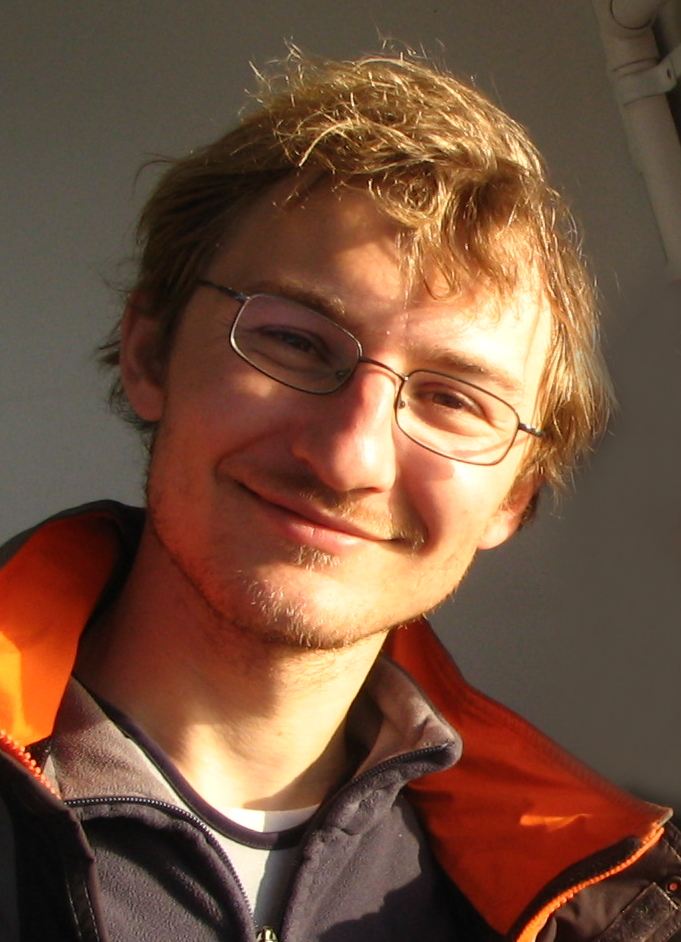
\includegraphics[height=3\baselineskip]{Thomas}&
		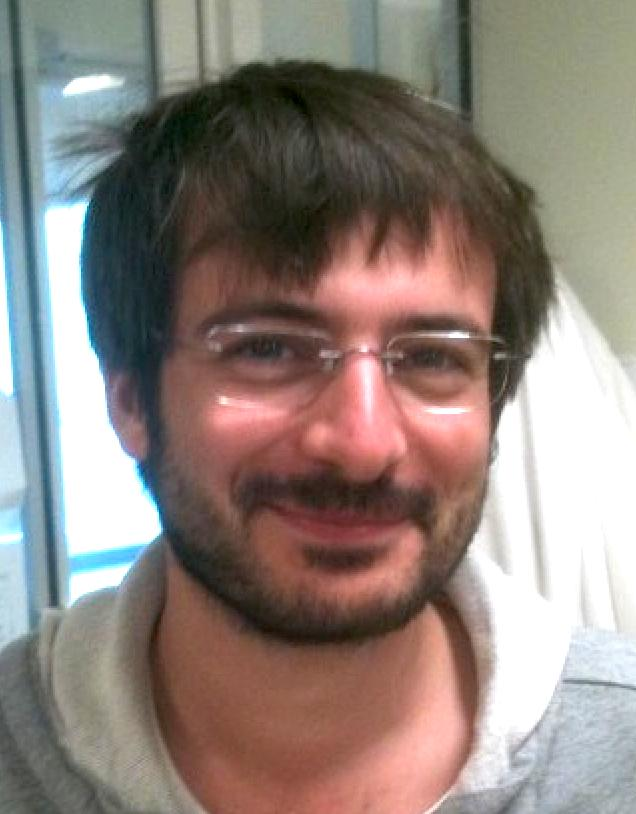
\includegraphics[height=3\baselineskip]{Thibaut}&
		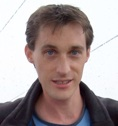
\includegraphics[height=3\baselineskip]{Seb}\\
		Christophe Perge & Thomas\linebreak Gibaud & Thibaut\linebreak Divoux & Sebastien Manneville\\
	\end{tabu}
	
	\vfill
	
\includegraphics[height=2\baselineskip,clip=true, trim=6mm 14mm 6mm 0]{NEW-Logo-ERC-OUTLINE}\quad
	
\includegraphics[height=2\baselineskip]{logo_ums_grand}\quad
	
\includegraphics[height=2\baselineskip]{CNRSfilaire-Q}\quad
	
\includegraphics[height=2\baselineskip]{CRPP}\quad
	
\includegraphics[height=2\baselineskip]{logo_ens-lyon}
	}



\newlength{\mylength}

%\includeonly{creep_beamer}

\begin{document}
\tikzset{every mark/.append style={scale=0.8}}
\pgfplotsset{every axis/.append style={footnotesize}}

\pgfplotscreateplotcyclelist{earthy}{%
red!40!black,
red!60!black,
red!80!black,
red,
red!80!yellow,
red!60!yellow,
red!40!yellow,
}

\AtBeginSection[]{
	\addtocounter{framenumber}{-1}
	\begin{frame}[plain]
		\tableofcontents[currentsection, hideothersubsections]
	\end{frame}
}

\begin{frame}[plain]
	\titlepage
\end{frame}

\setcounter{framenumber}{0}

\begin{frame}{Over-acidified protein gels: beyond isoelectric pH}
	
	Milk protein solution (4\%w sodium caseinate) acidified by the slow hydrolysis of glucono-$\delta$-lactone (\textsc{gdl})\\ %\textit{Bremer et al., Colloids Surf. (1990); van Vliet \& Walstra, Faraday Discuss. (1995); Lucey \& Singh, Food Res. Int. (1997); Leocmach et al. PRL (2014)}
	
	\smallskip
	\tikzsetnextfilename{prise_cas4}
	\begin{tikzpicture}
\pgfplotsset{every axis/.append style={xlabel absolute, every axis x label/.append style={anchor=base, yshift=-1em}, ylabel absolute, every axis y label/.append style={anchor=base, yshift=0em}}}

\begin{groupplot}[
	group style={
			group name=g, group size=1 by 2,
			vertical sep=0.5em,
			x descriptions at=edge bottom,
		},
	scale only axis,
	width=0.8\textwidth,
	height=4\baselineskip,
	xlabel={time (h)}, 
	xmin=0, xmax=4.5,
	extra tick style={grid=major},%
	]

 %%%% pH %%%%
\nextgroupplot[
	ymin=0, ymax=7, ylabel={pH},
	extra y ticks={4.6}, extra y tick labels={},%
	cycle list name=earthy,
	no marks,
	xmin=0, xmax=20,xtick={0,2,...,20},
	]
	\begin{scope}[every node/.style={anchor=base west, inner xsep=0, font=\small}]
	\addplot table[x expr={\thisrowno{0}/3600.+0.05}]{Y190_cas4_gdl1.pH}  (axis cs:20,4) node[below left] {\textsc{gdl} 1\%};
	\pgfplotsset{cycle list shift=4};
	\addplot table[x expr={\thisrowno{0}/3600.+0.05}]{Y189_28800s.pH}  node {\textsc{gdl} 4\%};
	\end{scope}
	\node[base left=0] at (axis cs:17,4.6) {isoelectric};



 %%%% prise unscaled %%%%
\nextgroupplot[
	height=6\baselineskip,
	ylabel={$G^\prime$ (\si{\pascal})},
	cycle list name=earthy,
	no marks,
	xmin=0, xmax=20,ymin=0,ymax=950,xtick={0,2,...,20},
	]
	\begin{scope}[every node/.style={anchor=base west, inner xsep=0, font=\small}]
	\addplot table[x expr={\thisrowno{0}/3600}]{cas4_GDL1_Y265.prise} node {1\%};
	\addplot table[x expr={\thisrowno{0}/3600}]{cas4_GDL1.25_Y277.prise} node {1.25\%};
	\addplot table[x expr={\thisrowno{0}/3600}]{cas4_GDL1.5_Y275.prise} node {1.5\%};
	\addplot table[x expr={\thisrowno{0}/3600}]{cas4_GDL2_Y268.prise} node[yshift=0.1em] {2\%};
	\addplot table[x expr={\thisrowno{0}/3600}]{cas4_GDL3_Y270.prise} node[yshift=-0.1em] {3\%};
	\addplot table[x expr={\thisrowno{0}/3600}]{cas4_GDL4_Y271.prise} node[yshift=-0.5em] {4\%};
	\end{scope}
	\draw[->, thick] (axis cs: 14,850) -- (axis cs:12,60) node[pos=0.25, right]{\textsc{gdl}$\searrow$};

\end{groupplot}

\end{tikzpicture}
	\begin{itemize}
	\item Caseins regain charges, solubility below isoelectric $\Rightarrow$ $G^\prime\searrow$
	\item The sample is still solid
	\end{itemize}
\end{frame}

\begin{frame}{Linear rheology, from power-law to soft glassy}
	\tikzsetnextfilename{sweep_cas4}
	\begin{figure}
\begin{tikzpicture}
\pgfplotstableread{freqsweep_Y265_cas4_GDL1.txt}\GDLa
\pgfplotstableread{freqsweep_Y277_cas4_GDL1.25.txt}\GDLb
\pgfplotstableread{freqsweep_Y275_cas4_GDL1.5.txt}\GDLc
\pgfplotstableread{freqsweep_Y268_cas4_GDL2.txt}\GDLd
\pgfplotstableread{freqsweep_Y270_cas4_GDL3.txt}\GDLe
\pgfplotstableread{freqsweep_Y271_cas4_GDL4.txt}\GDLf

\begin{groupplot}[
	group style={
			group name=g, group size=2 by 2,
			vertical sep=2.5em,
			horizontal sep=4em,
			%xticklabels at=edge bottom,
		},
	scale only axis,
	width=0.6\columnwidth-4em,
	height=4\baselineskip,
	domain={6e-2:70},
	cycle list name=earthy,
	xmode=log, ymode=log,
	xmin=5e-2, xmax=1e3,
	xlabel={$f$ (\si{\hertz})},
	xlabel absolute, every axis x label/.append style={anchor=base, yshift=-0.5em},
	]

%%%%Elastic%%%%
\nextgroupplot[ylabel={$G^\prime$ (\si{\pascal})}, ymin=18, ymax=3e3, no marks]
\begin{scope}[
	every axis plot post/.append style={only marks, mark=*, mark options={scale=0.1}},
	every node/.style={anchor=west, ,font=\scriptsize, pos=0}
]
	\addplot table{\GDLa} node[anchor=base west]{1\%};
	\addplot table{\GDLb} node[anchor=base west]{1.25\%};
	\addplot table{\GDLc} node[yshift=0.1em]{1.5\%};
	\addplot table{\GDLd} node[yshift=0.1em]{2\%};
	\addplot table{\GDLe} node{3\%};
	\addplot table{\GDLf} node[yshift=-0.2em]{4\%};
\end{scope}
\pgfplotsset{cycle list shift=-6}
\addplot {590.277*x^0.139256};
\addplot {349.762*x^0.121815};
\addplot {246.573*x^0.102707};
\addplot {162.851*x^0.0676911};
\addplot {109.351*x^0.0437222};
\addplot {76.7364*x^0.035779};
\draw[->, thick] (axis cs: 7,850) -- (axis cs:12,60) node[pos=0, anchor=south east]{\textsc{gdl}$\searrow$};

%%%Exponent%%%
\nextgroupplot[
	width=0.4\columnwidth-4em-5pt,
	xlabel={GDL (\%)},
	xmode=linear,
	ymode=linear,
	xmin=0, xmax=4.5,
	ylabel={exponent}, ymin=0,ymax=0.15,
	ytick={0,0.05,0.1}, yticklabels={0,0.05,0.10},
]
\addplot[mark=*] file{sweep_exponents.txt};


%%%Loss%%%
\nextgroupplot[ylabel={$G^{\prime\prime}$ (\si{\pascal})}, ymin=3, ymax=5e2, no marks]
\begin{scope}[
	every axis plot post/.append style={only marks, mark=*, mark options={scale=0.1}},
	every node/.style={anchor=west,font=\scriptsize, pos=0}
]
	\addplot table[y index=2]{\GDLa} node{1\%};
	\addplot table[y index=2]{\GDLb} node{1.25\%};
	\addplot table[y index=2]{\GDLc} node[yshift=-0.1em]{1.5\%};
	\addplot table[y index=2]{\GDLd} node{2\%};
	\addplot table[y index=2]{\GDLe} node{3\%};
	\addplot table[y index=2]{\GDLf} node[yshift=-0.2em]{4\%};
\end{scope}
\pgfplotsset{cycle list shift=-6}
\addplot {140.022*x^0.139256};
\addplot {72.4462*x^0.121815};
\addplot {43.0813*x^0.102707};
\addplot {18.9117*x^0.0676911};
\addplot {8.39838*x^0.0437222};
\addplot {4.99978*x^0.035779};
\draw[->, thick] (axis cs: 7,200) -- (axis cs:12,4) node[pos=0, above left=-0.5em and 0]{\textsc{gdl}$\searrow$};

\nextgroupplot[
	width=0.4\columnwidth-4em-5pt, 
	ylabel={$G^{\prime\prime}/G^{\prime\prime}_{\SI{1}{\hertz}}$}, 
	ymode=linear, ymin=0.5,
	xmin=0.05,xmax=100, xtick={0.1,1,10},
	%xmin=0, xmax=60,
	no marks,
]
\begin{scope}[
	%every axis plot post/.append style={mark=*, mark options={scale=0.1}},
	every node/.style={anchor=west,font=\scriptsize, pos=0}
]
	\addplot table[y expr={\thisrowno{2}/140.022}]{\GDLa} node[pos=0.25,left]{1\%};
	\addplot table[y expr={\thisrowno{2}/72.4462}]{\GDLb};
	\addplot table[y expr={\thisrowno{2}/43.0813}]{\GDLc};
	\addplot table[y expr={\thisrowno{2}/18.9117}]{\GDLd};
	\addplot table[y expr={\thisrowno{2}/8.39838}]{\GDLe};
	\addplot table[y expr={\thisrowno{2}/4.99978}]{\GDLf}node[pos=0.25,right]{4\%};
\end{scope}
\draw[->, thick] (axis cs: 20,1.8) -- (axis cs:60,1.2) node[pos=0, above left=-0.5em and 0]{\textsc{gdl}$\searrow$};
\end{groupplot}
\let\GDLa\relax
\let\GDLb\relax
\let\GDLc\relax
\let\GDLd\relax
\let\GDLe\relax
\let\GDLf\relax
\end{tikzpicture}
\end{figure}
	\begin{itemize}
	\item Near isoelectric, power law rheology $G^\prime, G^{\prime\prime}$ typical of gels 
	\item Over-acidification lowers exponent and creates a minimum in $G^{\prime\prime}$
	\item Transition to soft-glassy behaviour \\\textit{\footnotesize Sollich, PRE (1998); Mason, Curr. Opin. Colloid Interface Sci. (1999)}
	\end{itemize}
\end{frame}

\begin{frame}{Questions}
\begin{description}
\item[What] is the change in microstructure?
\item[How] does it affects the failure mechanism?
\end{description}
\end{frame}

\begin{frame}{Microscructure: fluorescent confocal microscopy}
	\tikzsetnextfilename{structure_confocal}
	\begin{tikzpicture}[every axis/.style={xlabel absolute, every axis x label/.append style={anchor=base, yshift=-1em}}]
\begin{groupplot}[
	group style={
			group name=g, group size=1 by 3,
			vertical sep=0.5em,
			xticklabels at=edge bottom,
		},
	scale only axis,
	height=3.5\baselineskip,
	width=0.5\textwidth-3em,
	xmin=0, xmax=8, ymin=0,
	cycle list name=earthy,
	no marks,
	]
\nextgroupplot[ylabel={$\xi$ (\si{\micro\metre})}, height=3\baselineskip, ymax=10, ytick={0,3,6,9}]
\addplot table[skip coords between index={0}{64}, x expr={\thisrowno{0}/3600.}, y expr={6.28*\thisrowno{1}}]{ech17_pore_size.txt};
\pgfplotsset{cycle list shift=4};
\addplot table[skip coords between index={0}{2}, x expr={\thisrowno{0}/3600}, y expr={6.28*\thisrowno{1}}]{ech26_pore_size.txt};

\nextgroupplot[ylabel={$\chi$ (a.u.)}]
\begin{scope}%[every node/.style={anchor=base west}]
\addplot table[skip coords between index={0}{64}, x expr={\thisrowno{0}/3600}, y expr={\thisrowno{2}/1e3}]{ech17_pore_size.txt} node[anchor=north east, pos=0.65] (l1) {\textsc{gdl} 1\%};
\pgfplotsset{cycle list shift=4};
\addplot table[x expr={\thisrowno{0}/3600}, y expr={\thisrowno{2}/2e3}]{ech26_pore_size.txt} node[anchor=base west, pos=0.3] {\textsc{gdl} 4\%};
\end{scope}

\nextgroupplot[xlabel={time (\si{\hour})}, ylabel={$d$}]
\addplot table[skip coords between index={0}{64}, x expr={\thisrowno{0}/3600}, y index=3]{ech17_pore_size.txt};
\pgfplotsset{cycle list shift=4};
\addplot table[x expr={\thisrowno{0}/3600}, y index=3]{ech26_pore_size.txt};
\node[anchor=south east, font=\scriptsize] at (rel axis cs:1,0) {$\displaystyle I(q) = \frac{2\chi\Gamma(d)}{\left(1+\left((d+1)\xi q\right)^2\right)^{d/2}}$};
\end{groupplot}


\matrix[matrix of nodes, inner sep=0, row sep=0.2em, column sep=0.2em, matrix anchor=north west] 
at ($(g c1r1.right of north east)+(-\textwidth,0)$)
(m) {
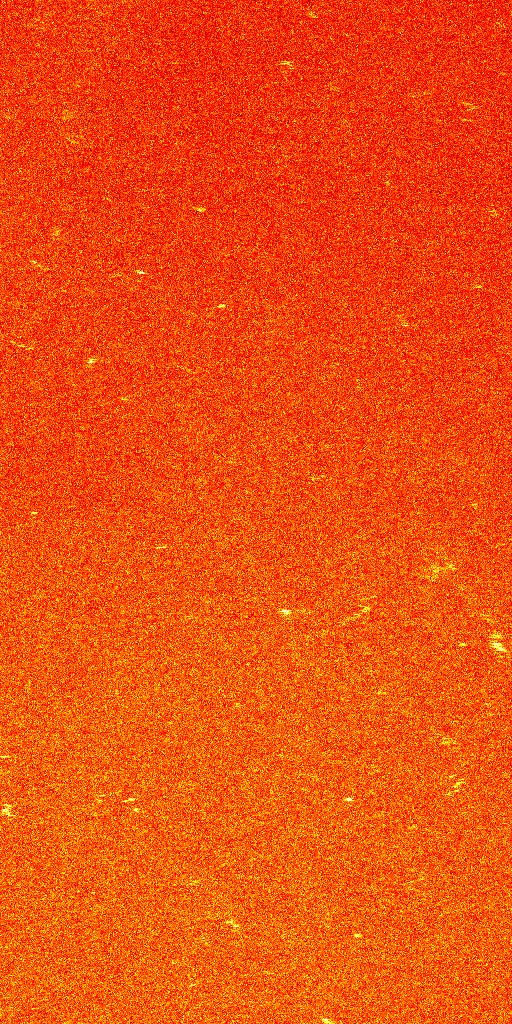
\includegraphics[width=2.5\baselineskip]{ech26_t00.jpg}&
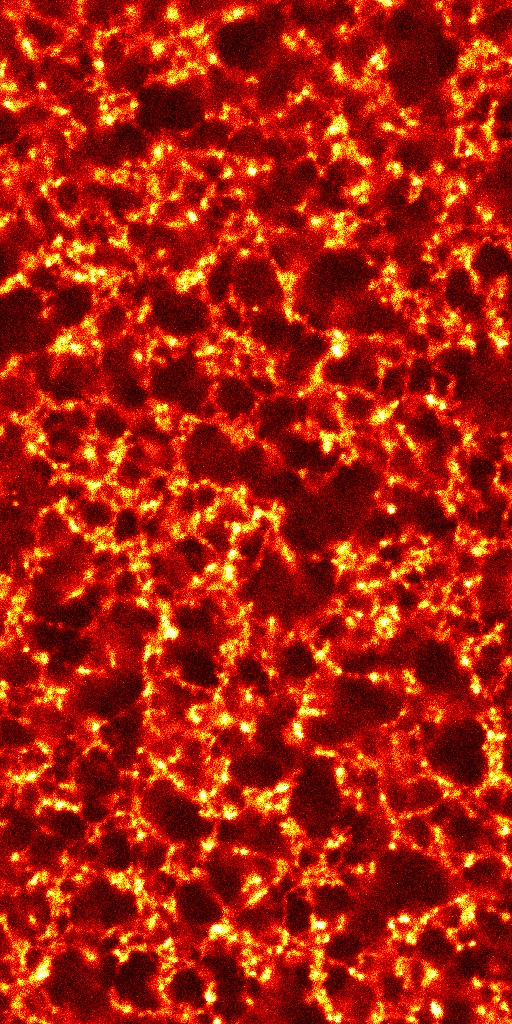
\includegraphics[width=2.5\baselineskip]{ech26_t05.jpg}&
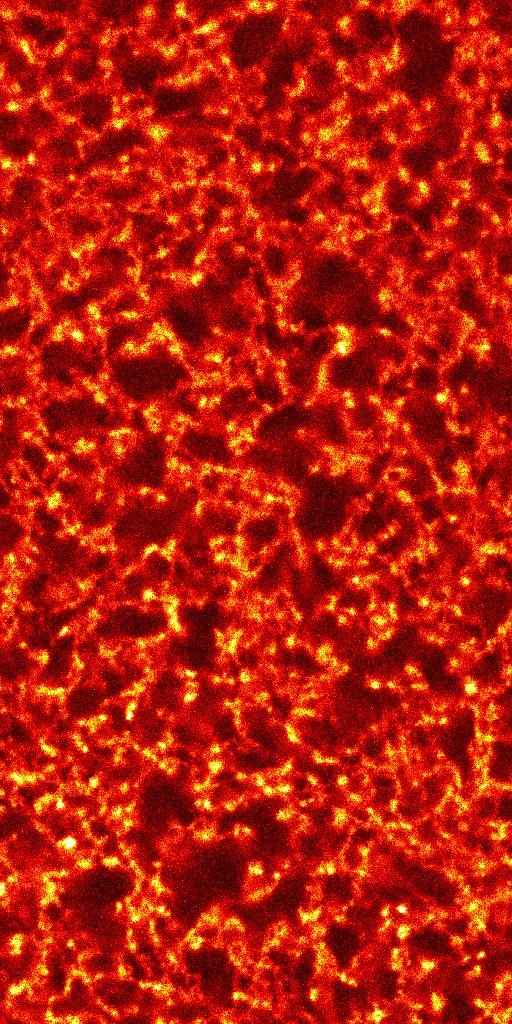
\includegraphics[width=2.5\baselineskip]{ech26_t30.jpg}&
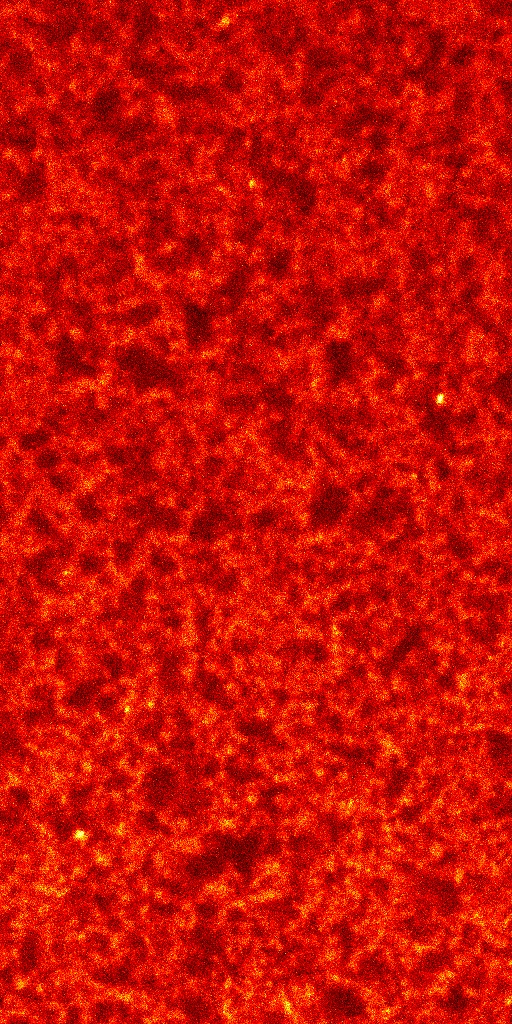
\includegraphics[width=2.5\baselineskip]{ech26_t70.jpg}\\
\SI{5}{\minute} & \SI{27}{\minute} & \SI{49}{\minute} & \SI{8}{\hour}\\
};
\draw[ultra thick, white] (m-1-1.south east) ++(-0.25\baselineskip,1em) -- +(-2\baselineskip,0) node[midway, above] {\SI{20}{\micro\metre}};

\newdimen\mydima
\newdimen\mydimb
\pgfextracty{\mydima}{\pgfpointanchor{g c1r1}{north}}
\pgfextracty{\mydimb}{\pgfpointanchor{g c1r3}{south}}
\begin{loglogaxis}[
	name=Sq,
	scale only axis,
	width=0.3\textwidth,
	height=4.5\baselineskip,
	anchor=left of south west,
	at={($(g c1r3.right of south east)+(-\textwidth,0)$)},
	cycle list name=earthy,
	xlabel={$q$ (\si{\per\micro\metre})},
	ylabel={$I(q)$ (a.u.)},
	domain=0.3:10,
	xmin=0.08, xmax=4e3,
	ymin=1e2, ymax=2e4,
	clip mode=individual,
	]
\begin{scope}[
	every axis plot post/.append style={only marks, mark options={scale=0.3}},
]
\addplot table{ech26_t00.Sq};
\addplot table{ech26_t02_4.Sq};
\addplot table{ech26_t02_5.Sq};
\addplot table{ech26_t02_6.Sq};
\addplot table{ech26_t02_7.Sq};
\addplot table{ech26_t03.Sq};
%\addplot table{ech26_t70.Sq};

\pgfplotsset{cycle list shift=-7}
\addplot table[x expr={100*\thisrowno{0}}]{ech26_t04.Sq};
\addplot table[x expr={100*\thisrowno{0}}]{ech26_t14.Sq};
\addplot table[x expr={100*\thisrowno{0}}]{ech26_t30.Sq};
\addplot table[x expr={100*\thisrowno{0}}]{ech26_t49.Sq};
\pgfplotsset{cycle list shift=4}
\addplot table[x expr={100*\thisrowno{0}}]{ech26_t70.Sq};
\end{scope}
\pgfplotsset{cycle list shift=-3}
\addplot+[domain=0.3:5] {433/(1+(1.69 * x)^2)^(0.24)} coordinate[pos=0] (t0);
\addplot {659/(1+(0.82 * x)^2)^(0.33)};
\addplot {1094/(1+(0.32 * x)^2)^(0.72)};
\addplot {2610/(1+(0.37 * x)^2)^(0.91)};
\addplot {4217/(1+(0.45 * x)^2)^(0.95)};
\addplot {7686/(1+(0.59 * x)^2)^(0.99)} coordinate[pos=0] (t1);
\pgfplotsset{cycle list shift=-2}
\addplot+[domain=30:1000] {9658/(1+(0.61e-2 * x)^2)^(0.98)} coordinate[pos=0] (t2);
\addplot+[domain=30:1000] {9652/(1+(0.60e-2 * x)^2)^(1.00)};
\addplot+[domain=30:1000] {6749/(1+(0.49e-2 * x)^2)^(1.07)};
\addplot+[domain=30:1000] {3797/(1+(0.43e-2 * x)^2)^(1.10)};
\pgfplotsset{cycle list shift=1}
\addplot+[domain=30:1000] {3111/(1+(0.44e-2 * x)^2)^(1.04)} coordinate[pos=0] (t3);

\draw[->, line width=0.2em] (t0) -- (t1) node[midway,rotate=90, above] {time};
\draw[->, line width=0.2em] (t2) -- (t3) node[midway,rotate=90, above] {time};

\end{loglogaxis}
\node[anchor=south west] at (Sq.outer south west) (gdl) {\textcolor{red!60!yellow}{\textsc{gdl} 4\%}};

\end{tikzpicture}

	\begin{itemize}
	\item Maximum $G^\prime$ corresponds to maximum contrast between phases
	\item Characteristic size $\xi$ increases during over-acidification
	\item Casein aggregates swell $\sim$ over compressed gel $\Rightarrow$ soft glassy
	\end{itemize}
\end{frame}

\begin{frame}{Three creep regimes + softness\hfill\textsc{gdl} 4\%}
\vfill
	\tikzsetnextfilename{creep_cas4_gdl4}
	\begin{tikzpicture}
\pgfplotsset{every axis/.append style={xlabel absolute, every axis x label/.append style={anchor=base, yshift=-0.5em}}, ylabel absolute, every axis y label/.append style={anchor=base, yshift=-1em}}
\begin{groupplot}[
	group style={
			group name=g, group size=2 by 2,
			horizontal sep=4em,
			%xticklabels at=edge bottom,
		},
	width=0.35\textwidth,
	height=8\baselineskip,
	cycle list name=earthy,
	xmode=log, ymode=log,
	%xmin=5e-2, xmax=1e3,
	ylabel={$\dot{\gamma}/\dot{\gamma}_\text{min}$},
	extra tick style={grid=major},%
	]
\nextgroupplot[
	xlabel={$t$ (\si{\second})}, ylabel={$\gamma$}, 
	ymax=3, ymin=2e-1,xmin=0.3,xmax=1e6,
	xtick={1, 1e2, 1e4, 1e6},
	ytick={0.1,0.2,0.4,0.8,1.6}, yticklabels={0.1,0.2,0.4,0.8,1.6},
	extra y ticks={1}, extra y tick labels={},]
\begin{scope}[every node/.style={font=\scriptsize, anchor=north west, inner xsep=0}]
\addplot table {Y242_20Pa_gamma_decimated.txt} node[pos=0.4, rotate=35, yshift=0.3em] {\SI{20}{\pascal}};
\addplot table {Y239_40Pa_gamma_decimated.txt} node[pos=0.3, rotate=30, yshift=0.2em] {\SI{40}{\pascal}};
\addplot table {Y238_50Pa_gamma_decimated.txt} node[anchor=south east, rotate=90] at (rel axis cs:0.78,1) {\SI{50}{\pascal}};
\addplot table {Y246_60Pa_gamma_decimated.txt} node[anchor=south east, rotate=90] at (rel axis cs:0.6,1) {\SI{60}{\pascal}};
\addplot table {Y236_100Pa_gamma_decimated.txt} node[pos=0.1, rotate=15, yshift=0.2em] {\SI{100}{\pascal}};
\addplot+[restrict x to domain=0.05:100] table {Y249_120Pa_gamma_decimated.txt} node[anchor=north east, rotate=80] at (rel axis cs:0.15,1) {\SI{120}{\pascal}};
\end{scope}

%%%Regime 1%%%
\nextgroupplot[
	xlabel={$t/\tau_f$},xmin=1e-5, xmax=2, xtick={1e-4, 1e-2, 1},
	ymin=0.5, ymax=5e4]
\addplot table {Y242_20Pa_gdot_decimated.txt};
\addplot table {Y239_40Pa_gdot_decimated.txt};
\addplot table {Y238_50Pa_gdot_decimated.txt};
\addplot table {Y246_60Pa_gdot_decimated.txt};
\addplot table {Y236_100Pa_gdot_decimated.txt};
\addplot+[restrict x to domain=-2.75:1] table {Y249_120Pa_gdot_decimated.txt};
\addplot[domain=1e-3:1e-1] {x^(-0.96)} node[pos=0, right] {-0.96};



%%%Regime2 %%%
\nextgroupplot[
	xlabel={$t/\tau_f$}, xmode=linear, ymode=linear, 
	xmin=0, xmax=1,ymin=0.5,ymax=10, restrict y to domain=0:11,
	xtick={0, 0.2, ..., 1}, ytick={2,4,6,8}]
\addplot table {Y242_20Pa_gdot_decimated.txt};
\addplot table {Y239_40Pa_gdot_decimated.txt};
\addplot table {Y238_50Pa_gdot_decimated.txt};
\addplot table {Y246_60Pa_gdot_decimated.txt};
\addplot table {Y236_100Pa_gdot_decimated.txt};
\addplot table {Y249_120Pa_gdot_decimated.txt};


%%%Regime 3%%%
\nextgroupplot[
	xlabel={$1-t/\tau_f$},xmin=1e-5, xmax=2, x dir=reverse, xtick={1e-4, 1e-2, 1},
	ymin=0.5, ymax=5e4]
\addplot table[x expr={1-\thisrowno{0}}] {Y242_20Pa_gdot_decimated.txt};
\addplot table[x expr={1-\thisrowno{0}}] {Y239_40Pa_gdot_decimated.txt};
\addplot table[x expr={1-\thisrowno{0}}] {Y238_50Pa_gdot_decimated.txt};
\addplot table[x expr={1-\thisrowno{0}}] {Y246_60Pa_gdot_decimated.txt};
\addplot table[x expr={1-\thisrowno{0}}] {Y236_100Pa_gdot_decimated.txt};
\addplot table[x expr={1-\thisrowno{0}}] {Y249_120Pa_gdot_decimated.txt};
\addplot[domain=1e-4:1e-2] {0.1*x^(-1)} node[midway, below] {-1};
\end{groupplot}
\node[below right] (Andrade) at (g c2r1.north west){Andrade creep $\Leftarrow$ power-law rheology};
\node[below right] (Finite) at (g c2r2.north west){Finite time div.  $\Leftarrow$ fracture growth};
\draw[<->, ultra thick, Accent1] (Andrade) -- (Andrade|-Finite.north) node [midway, right, text width=0.25\textwidth]{\textit{\footnotesize Leocmach et. al,\linebreak PRL (2014)}};
\node[anchor=north east, text width=0.35\textwidth] at (Finite.south-|Andrade.east) {
\begin{itemize}
		\item Erratic regime 2
		\item Possible to reform bonds? Glassy?
	\end{itemize}
};
\end{tikzpicture}
%	\begin{description}
%		\item[$\tau_f$] divergence of the strain
%		\item[$\tau_\text{min}$] minimum of shear rate $\dot{\gamma}$
%	\end{description}
%	\begin{itemize}
%		\item Erratic position of $\tau_\text{min}$
%		\item Possible to reform bonds? Glassy?
%	\end{itemize}
\begin{itemize}
%\item Failure scenario almost conserved: ``fibre bundle'' network
%\item Other dissipation due to softness: overcompressed gel
\item Prediction of failure from when fractures nucleate more difficult
\end{itemize}

\end{frame}


\begin{frame}[plain]
	\titlepage
\end{frame}

\appendix
\newcounter{finalframe}
\setcounter{finalframe}{\value{framenumber}}

\begin{frame}{Basquin law rescaling}
	\tikzsetnextfilename{basquin}
	\begin{tikzpicture}
\pgfplotsset{every axis/.append style={xlabel absolute, every axis x label/.append style={anchor=base, yshift=-0.5em}, ylabel absolute, every axis y label/.append style={anchor=base, yshift=-0.5em}}}
\begin{groupplot}[
	group style={
			group name=g, group size=2 by 2,
		    horizontal sep=6em,
			vertical sep=4em,
%			xticklabels at=edge bottom,
			%y descriptions at=edge left,
		},
	scale only axis,
	width=0.4\columnwidth-4em,
	xmode=log, ymode =log,
	ymax=2e6, xmin=0.125, xmax=2,
	xlabel=$\sigma/G^\prime$,
	ylabel={$\tau_\text{min}$ (\si{\second})},
	cycle list name=earthy,
	clip mode=individual,
	%cycle list shift=2,
	%ymin=0.01, ymax=1e6,
%	xmin=0, xmax=17, ymin=0,
%	cycle list name=linestyles,
%	no marks,
	]

%composition
\nextgroupplot[xlabel={$\sigma$ (\si{\pascal})}, xmin=10, xmax=2e3, ymin=2e-2, ytickten={-1,1,3,5}]
%\pgfplotsset{cycle list shift=3}
\addplot+[only marks, mark=square*] table[y index=5]{MCR_cas4_GDL1_gap10.txt} node[midway, above right] {1\%};
\addplot+[only marks, mark=square, black] table[y index=5]{MCR_cas4_GDL4_gap10.txt} node[midway, above right] {4\%};
%fits
\addplot[gray, domain=150:1000] {3.7e17*x^(-5.5)};
\addplot[gray, domain=20:350] {3.7e12*x^(-5.5)};

%composition rescaled
\nextgroupplot[xmax=4, ymin=2e-2, xtick={0.25, 0.5, 1, 2,4}, xticklabels={0.25, 0.5, 1, 2,4}, ytickten={-1,1,3,5}]
\addplot+[only marks, mark=square*] table[x expr={\thisrowno{0}/\thisrowno{2}}, y index=5]{MCR_cas4_GDL1_gap10.txt};
\addplot+[only marks, mark=square, black] table[x expr={\thisrowno{0}/\thisrowno{2}}, y index=5]{MCR_cas4_GDL4_gap10.txt};
%fit
\addplot[gray, domain=0.18:3.5] {40.6*x^(-5.5)} node[midway, below left] {-5.5};

%gap
\nextgroupplot[xtick={0.25, 0.5, 1}, xticklabels={0.25, 0.5, 1}, ymin=8]
\begin{scope}[every node/.style={inner xsep=0, font=\small}]
\addplot+[only marks, mark=square*] table[x expr={\thisrowno{0}/\thisrowno{2}}, y index=5]{MCR_cas4_GDL1_gap10.txt} node[pos=0, above right] {$e=\SI{1}{\milli\metre}$};
\pgfplotsset{cycle list shift=2}
\addplot+[only marks, mark=diamond*] table[x expr={\thisrowno{0}/\thisrowno{2}}, y index=5]{MCR_cas4_GDL1_gap15.txt} node (los){} node[above left] (lablos) at (rel axis cs:1, 0.6) {$e=\SI{1.5}{\milli\metre}$} [->] (lablos.base west) -| (los);
\pgfplotsset{cycle list shift=4}
\addplot+[only marks, mark=*] table[x expr={\thisrowno{0}/\thisrowno{2}}, y index=5]{MCR_cas4_GDL1_gap30.txt} node[below left] at (axis cs:0.5,1e2){$e=\SI{3}{\milli\metre}$};
\end{scope}
%fit
\addplot[gray, domain=0.2:1.3] {40.6*x^(-5.5)};
\addplot[gray, domain=0.17:0.5] {0.77*x^(-5.5)};

%gap rescaled
\nextgroupplot[ylabel={$\tau_\text{min} e^3$ (\si{\cubic\milli\metre\second})},xtick={0.25, 0.5, 1}, xticklabels={0.25, 0.5, 1}, ymin=8]
%\addplot+[only marks] table[x expr={\thisrowno{0}/\thisrowno{2}}, y expr={\thisrowno{5}*0.5^3}]{MCR_cas4_GDL1_gap05.txt};
%\pgfplotsset{cycle list shift=2}
\addplot+[only marks, mark=square*] table[x expr={\thisrowno{0}/\thisrowno{2}}, y expr={\thisrowno{5}*1^3}]{MCR_cas4_GDL1_gap10.txt};
\pgfplotsset{cycle list shift=2}
\addplot+[only marks, mark=diamond*] table[x expr={\thisrowno{0}/\thisrowno{2}}, y expr={\thisrowno{5}*1.5^3}]{MCR_cas4_GDL1_gap15.txt};
\pgfplotsset{cycle list shift=4}
\addplot+[only marks, mark=*] table[x expr={\thisrowno{0}/\thisrowno{2}}, y expr={\thisrowno{5}*3^3}]{MCR_cas4_GDL1_gap30.txt};
%fit
\addplot[gray, domain=0.15:1.3] {34.9*x^(-5.5)};
\end{groupplot}
\node[anchor=south west] at (g c1r1.north west) {\textcolor{Accent1}{$\blacktriangleright$} Composition rescaled by elastic modulus};
\node[anchor=south west] at (g c1r2.north west) {\textcolor{Accent1}{$\blacktriangleright$} Geometry rescaled as a fracture nucleation rate};
\end{tikzpicture}
\end{frame}

\begin{frame}{Monkman-Grant: Predict failure from nucleation}
	\tikzsetnextfilename{MonkmanGrant}
	\begin{tikzpicture}
\pgfplotsset{every axis/.append style={
	xlabel absolute, every axis x label/.append style={anchor=base, yshift=-0.5em}, 
	ylabel absolute, every axis y label/.append style={anchor=base, yshift=-0.5em},
	%scale only axis,
	width=0.5\textwidth,
	height=10\baselineskip,
	xmode=log, xmin=1, xmax=1e6,
	domain=1:1e6,
}}
\begin{axis}[
	name=a,
	ylabel={$\tau_\text{min}$ (\si{\second})}, ymode=log, ymin=1,
	legend pos=outer north east,
	legend style={font=\normalsize, fill=none, draw=none},
	xticklabels={}
]
\addplot[only marks, mark=*] table[x index=4, y index=5]{MCR_cas4_GDL1_gap10.txt};
\addlegendentry{1\%, $e=\SI{1}{\milli\metre},\, H=\SI{28}{\milli\metre}$};
\addplot[only marks, mark=square*] table[x index=4, y index=5]{MCR_cas4_GDL1_gap30.txt};
\addlegendentry{1\%, $\textcolor{Accent2}{e=\SI{3}{\milli\metre}},\, H=\SI{28}{\milli\metre}$};
\addplot[gray, only marks, mark=o] table[x index=4, y index=5]{ARG2_cas4_GDL1_gap20.txt};
\addlegendentry{1\%, $e=\SI{1}{\milli\metre},\, \textcolor{Accent2}{H=\SI{60}{\milli\metre}}$};
\addplot[red, only marks, mark=star] table[x index=4, y index=5]{MCR_cas4_GDL4_gap10.txt};
\addlegendentry{\textcolor{Accent2}{4\%}, $e=\SI{1}{\milli\metre},\, H=\SI{28}{\milli\metre}$};
\addplot[no marks]{0.6*x};
\addplot[no marks, dashed]{0.4*x};
\end{axis}

\begin{axis}[
	anchor=north west,
	at={(0,-0.5em)},
	xlabel={$\tau_f$ (\si{\second})},
	ylabel=$\tau_\text{min}/\tau_f$, ymin=0, 
]
\addplot[only marks, mark=*] table[x index=4, y expr={\thisrowno{5}/\thisrowno{4}}]{MCR_cas4_GDL1_gap10.txt};
\addplot[only marks, mark=square*] table[x index=4, y expr={\thisrowno{5}/\thisrowno{4}}]{MCR_cas4_GDL1_gap30.txt};
\addplot[gray, only marks, mark=o] table[x index=4, y expr={\thisrowno{5}/\thisrowno{4}}]{ARG2_cas4_GDL1_gap20.txt};
\addplot[red, only marks, mark=star] table[x index=4, y expr={\thisrowno{5}/\thisrowno{4}}]{MCR_cas4_GDL4_gap10.txt};
\addplot[no marks]{0.6};
\addplot[no marks, dashed]{0.4};
\end{axis}

\node[anchor=north east, text width=0.5\textwidth] at ($(a.left of south west)+(\textwidth,-0.5em)$) {
\begin{itemize}
\item 	Height-dependent near isoelectric
\item Upper bound for over-acidified
\end{itemize}};

%\node[inner sep=0] at ($(a.east)-(3\TPHorizModule,0)$) {};
%\draw (a.outer east) ++ (-3\TPHorizModule,0) -- +(0,-2\TPVertModule);
\end{tikzpicture}
\end{frame}

\begin{frame}{Wavelength}
	\tikzsetnextfilename{lambda}
	\begin{tikzpicture}
\pgfplotsset{every axis/.append style={xlabel absolute, every axis x label/.append style={anchor=base, yshift=-0.5em}, ylabel absolute, every axis y label/.append style={anchor=base, yshift=-1em}}}
\begin{groupplot}[
	group style={
			group name=g, group size=2 by 1,
			horizontal sep=0.5em,
%			xticklabels at=edge bottom,
			y descriptions at=edge left,
		},
	scale only axis,
	width=0.5\textwidth-2em,
	height=7\baselineskip,
	xmin=0, ymin=0,
	ylabel={$\lambda$ (\si{\milli\metre})},
]

\nextgroupplot[xlabel={$\sigma$ (\si{\pascal})}, xmax=900, xtick={0,200,...,800}]
\addplot[only marks, error bars/.cd, y dir=both, y explicit] table[y error=erreur]{lambda_sigma_cas4_GDL1_ARG2.txt};
\addplot[mark=o, only marks, error bars/.cd, y dir=both, y explicit] table[y error=erreur]{lambda_sigma_cas4_GDL4_ARG2.txt};
\addplot[no marks, domain=0:900] {2.61} node[pos=0.75, below] {1\%};
\addplot[no marks, dotted, domain=0:900] {3.25} node[pos=0.75, above] {4\%};

\nextgroupplot[xlabel={gap (\si{\milli\metre})}, xmax=3.5, cycle list name=earthy]
\addplot[mark=o, only marks, error bars/.cd, y dir=both, y explicit] table[x=gap, y=lambda, y error=erreur, restrict expr to domain={\thisrowno{0}}{20:26}]{lambda_gap_cas4GDL4.txt};
\addplot+[mark=*, only marks, error bars/.cd, y dir=both, y explicit] coordinates{(2,2.61) +- (0,0.34)} node[above left]{$H=\SI{60}{\milli\metre}$};
\pgfplotsset{cycle list shift=2};
\addplot+[mark=diamond*, only marks, error bars/.cd, y dir=both, y explicit] table[x=gap, y=lambda, y error=erreur, restrict expr to domain={\thisrowno{0}}{30:38}]{lambda_gap_cas4GDL4.txt} node[above left=0.5em] {$R=\SI{37}{\milli\metre}$};
\pgfplotsset{cycle list shift=3};
\addplot+[mark=triangle*, only marks, error bars/.cd, y dir=both, y explicit] table[x=gap, y=lambda, y error=erreur, restrict expr to domain={\thisrowno{0}}{38:50}]{lambda_gap_cas4GDL4.txt} node[below right] {$R=\SI{40}{\milli\metre}$};
\addplot[no marks, domain=0:4] {1.3*x};
%\addplot[only marks, error bars/.cd, y dir=both, y explicit] table[x=gap, y expr={\thisrow{lambda}}, y error=erreur]{lambda_gap_cas4GDL1.txt};

\end{groupplot}
\newdimen\mydima
%\pgfextractx{\mydima}{\pgfpointanchor{g c1r1}{north east}}
\mydima=0.75\textwidth
\node[inner sep=0, above left =0.5em and 0 of g c2r1.north east] (im) {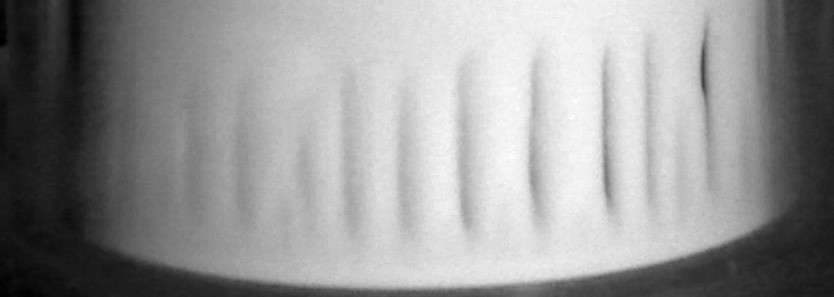
\includegraphics[width=\mydima]{Y140_bottom}};
\draw[<->] (im.north west) ++ (0.48\mydima, -0.2\mydima) -- +(0.075\mydima,0) node[midway,above] {$\lambda$};

%\draw (g c1r2.outer east) ++ (-3\TPHorizModule,0) -- +(0,2\TPVertModule);
\end{tikzpicture}

	\textcolor{Accent1}{$\blacktriangleright$} $\lambda\propto e$ compatible with nucleation rate

\end{frame}


\end{document}

